\documentclass[notheorems]{beamer}
\usetheme{Lab2C}
\usepackage{graphicx}
\usepackage{subcaption}
\usepackage{amsfonts}
\usepackage{amsmath}
\usepackage{amssymb}
\usepackage{amsthm}
\usepackage{algorithm}
\usepackage{algorithmic}
\usepackage{bm}
\usepackage{hyperref}
\usepackage{footmisc}
\usepackage{xcolor}




\DeclareMathOperator*{\argmin}{arg\,min}
\DeclareMathOperator*{\argmax}{arg\,max}
\DeclareMathOperator\E{\mathbb{E}}
\DeclareMathOperator\Var{\mathrm{Var}}
\def\R{\mathbb{R}}
\def\P{\mathcal{P}}
\usepackage{mathtools}
\DeclarePairedDelimiter\abs{\lvert}{\rvert}
\DeclarePairedDelimiter\norm{\lVert}{\rVert}
\DeclarePairedDelimiter\inner{\langle}{\rangle}
\DeclarePairedDelimiter\floor{\lfloor}{\rfloor}
\DeclarePairedDelimiter\ceil{\lceil}{\rceil}
\def\red#1{\textcolor{red}{#1}}
\makeatletter
\newcommand{\algorithmicfunction}{\textbf{function}}
\newcommand{\algorithmicendfunction}{\algorithmicend\ \algorithmicfunction}
\newenvironment{ALC@func}{\begin{ALC@g}}{\end{ALC@g}}
\newcommand{\FUNCTION}[2][default]{\ALC@it\algorithmicfunction\ #2\ %
\textbf{:}%
\ALC@com{#1}\begin{ALC@func}}
\ifthenelse{\boolean{ALC@noend}}{
    \newcommand{\ENDFUNCTION}{\end{ALC@func}}
  }{
    \newcommand{\ENDFUNCTION}{\end{ALC@func}\ALC@it\algorithmicendfunction}
  }
\makeatother
\theoremstyle{definition}
\newtheorem{definition}{Definition}
\newtheorem{theorem}{Theorem}
\newtheorem{example}{Example}
\newtheorem{proposition}{Proposition}
\newtheorem{corollary}{Corollary}
\newtheorem{lemma}{Lemma}
\newtheorem{remark}{Remark}

\newif\ifbeamer
\beamertrue

\title{Info-Detection: An Information-Theoretic Approach to Detect Outlier}
\author{Feng Zhao\inst{1} \and Fei Ma\inst{2}\and Yang Li\inst{2} \and Shao-Lun Huang\inst{2} \and Lin Zhang \inst{1,2}}
\institute{\inst{1}Dept. of Electronic Engineering, Tsinghua University
\and \inst{2}Tsinghua-Berkeley Shenzhen Institute, Tsinghua University}
\date{\today}
\begin{document}
\begin{frame}
	\titlepage
\end{frame}
\section*{Outline}
\begin{frame}
	\tableofcontents
\end{frame}

\section{Introduction}
\subsection{Outlier detection and existing method}
\begin{frame}
\frametitle{Outlier detection}
	\begin{columns}
		\column{5cm}
		\begin{figure}
			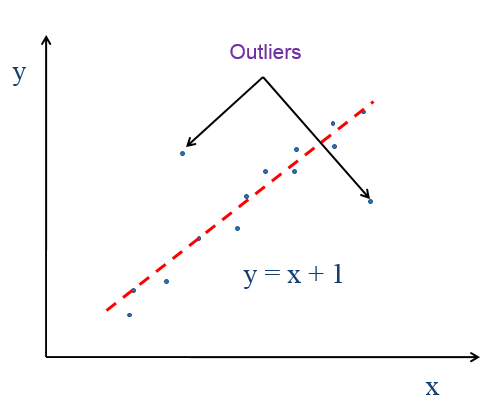
\includegraphics[width=4cm]{pic/outlier_detection_intro.png}
		\end{figure}
		\column{5cm}
		Outlier detection is the identification of abnormal data which differs from the majority of the data.
	\end{columns}
\begin{figure}
	\centering
	\begin{subfigure}{0.33\textwidth}
		
\includegraphics[width=\textwidth]{pic/fraud_detection.jpg}
		\caption{Fraud Detection}
	\end{subfigure}~~~~~
	\begin{subfigure}{0.33\textwidth}
		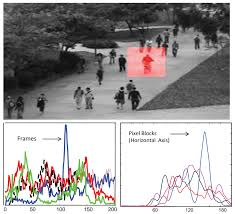
\includegraphics[width=\textwidth]{pic/activity_monitoring.jpg}
		\caption{Activity Monitoring}
	\end{subfigure}
\end{figure}  
\end{frame}
\begin{frame}
\frametitle{Existing Method}
\begin{figure}
	\centering
	\begin{subfigure}{0.33\textwidth}
		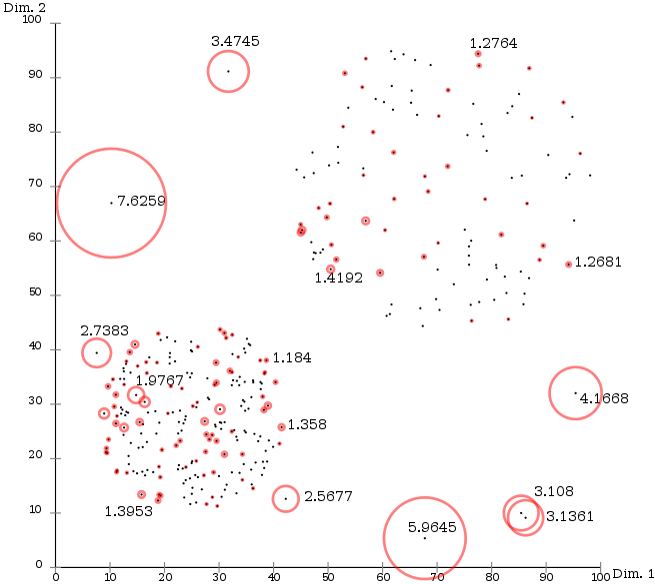
\includegraphics[width=\textwidth]{pic/lof.png}
		\caption{Local Outlier Factor}
	\end{subfigure}~
	\begin{subfigure}{0.58\textwidth}
		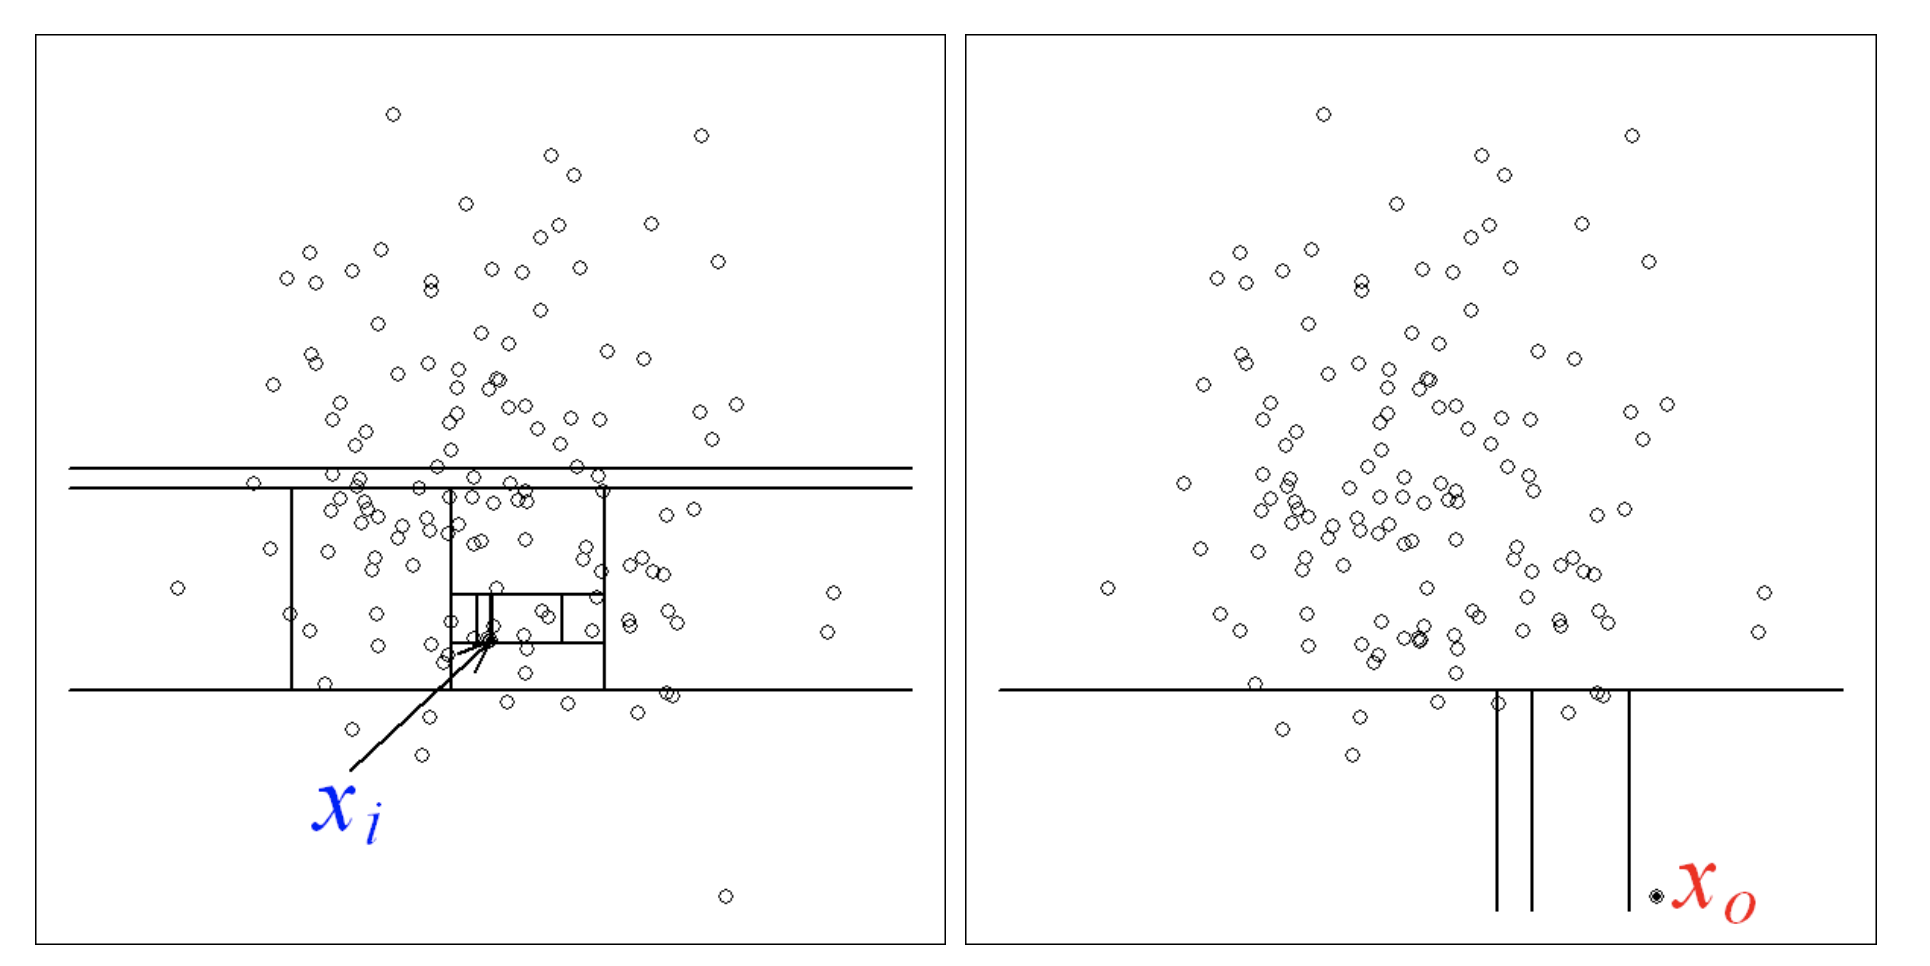
\includegraphics[width=\textwidth]{pic/if.png}
		\caption{Isolation Forest}
	\end{subfigure}
\end{figure}  
	\begin{columns}
\column{0.4\textwidth}
\begin{figure}
		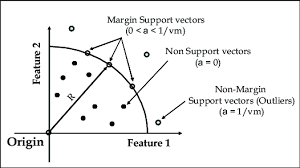
\includegraphics[width=4.5cm]{pic/one_class_svm.png}
		\caption*{ \textcolor{thupurple}{(c)} One class SVM}
\end{figure}
\column{0.6\textwidth}
\quad Shortcomings:
\begin{itemize}
\item the number of outliers needs to known 
\item hyperparameters matter
\end{itemize}
\end{columns}
\end{frame}
\begin{frame}
	\frametitle{Related work}
\begin{itemize}
\item Cluster based method
	\begin{enumerate}
		\item Campello et al. in 2015 proposed a hierarchical density estimate method
%to do outlier detection
		\item Nagano et al in 2010 proposed a minimum average cost clustering method
%which shares the same hierarchical clustering structure with info-clustering.
		\item Chan C et al. in 2016 proposed info-clustering method
%which is a hierarchical clustering method.
	\end{enumerate}
\item Graph partition algorithm
\begin{enumerate}
\item Narayanan in 1991 proposes an algorithm to compute the principal sequence of partition
\item Kolmogorov in 2010 proposes a parametric algorithm for the same task.
\end{enumerate}
\end{itemize}
Our work
\begin{itemize}
\item Info-Detection method
\item Improved algorithm for principal sequence of partition
\end{itemize}
\end{frame}
\subsection{Mutual similarity and its extension}
\begin{frame}
\begin{block}{mutual similarity}
\begin{itemize}
\item Gaussian kernel $ \exp({-\gamma \norm{p_1 - p_2}^2})$
\item threshold distance $\delta(\norm{p_1-p_2} < \delta^*)$
\end{itemize}
\end{block}
Notation:  $\P=\{C_1, \dots, C_k\}, \bigcup_{i=1}^k C_i = V$ and $i\neq j \Rightarrow C_i \cap C_j = \emptyset$
$\Pi$ is the collection of all partitions of $V$, $\Pi' = \Pi \backslash \{V\}$.
\begin{definition}[Multivariate Similarity]
Given a graph $G(V, E)$, with vertex as data point, edge weight as mutual similarity, the multivariate similarity $I(Z_V)$
\begin{align}
I(Z_V) & = \min_{\mathcal{P} \in \Pi'(V)} I_{\mathcal{P}}(Z_V) \\
\label{eq:newDef}  I_{\mathcal{P}}(Z_V) & = \frac{1}{ \abs{\mathcal{P}} - 1} \sum_{\substack{i\in C, j \not\in C\\ C\in \mathcal{P}, (i,j) \in E}} w_{ij}
\end{align}
\end{definition}
\end{frame}


\begin{frame}{Hierarchical clustering method}
\begin{description}
\item[top-down] $I_{\P^*}(Z_V)=I(Z_V)$ and use $\P^*$ to split.
\item[bottom-up] $I(Z_C) = \max_{B\subseteq V} I(Z_B)$ and use $C$ to merge.
\end{description}
\begin{figure}
\centering
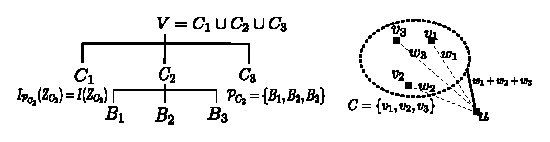
\includegraphics[width=\textwidth]{pic/two_approach.eps}
\caption{Left: top-down approach. Right: bottom-up approach}
\end{figure}
\end{frame}
\begin{frame}
	\frametitle{Illustrative example}
	\begin{columns}
		\column{5cm}
		\begin{figure}
			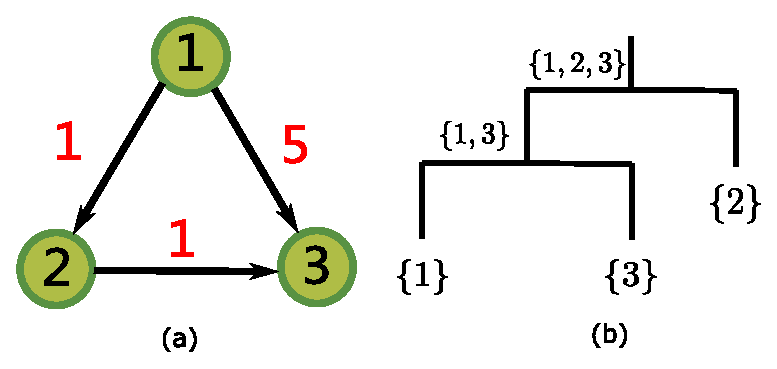
\includegraphics[width=4cm]{pic/example_directed.eps}
		\end{figure}
		\column{5cm}
		\begin{align*}
			I_{\{1\},\{2\},\{3\}}(Z_{\{1,2,3\}}) & = 3.5 \\
			I_{\{1,3\},\{2\}}(Z_{\{1,2,3\}}) & = 2 \\ 
			I_{\{1,2\},\{3\}}(Z_{\{1,2,3\}}) & = 6 \\ 
			I_{\{1\},\{2,3\}}(Z_{\{1,2,3\}}) & = 6 \\ 
			\Rightarrow I(Z_{\{1,2,3\}}) & = 2 \\
		\end{align*}
		\begin{equation*}
			I(Z_{\{1,3\}}) = 5, I(Z_{\{1,2\}}) = 1
		\end{equation*}
	\end{columns}
\end{frame}
\subsection{Examples}
\begin{frame}
\begin{figure}
\centering
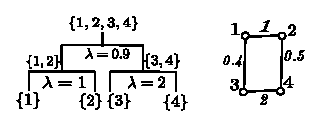
\includegraphics[width=0.7\textwidth]{pic/threshold.eps}
\caption{a clustering tree (left) for the weighted graph (right)}
\end{figure}

The threshold values $\lambda$ are $I(Z_{3,4})=2, I(Z_{1,2})=1$ and $I(Z_V)=0.9$ respectively.
\begin{equation*}
\P = 
\begin{cases}
\{\{1,2,3,4\}\} & \lambda < 0.9 \\
\{\{1,2\},\{3,4\}\} & 0.9 \leq \lambda < 1 \\
\{\{1\},\{2\},\{3,4\}\} & 1 \leq \lambda < 2\\
\{\{1\},\{2\},\{3\},\{4\}\} & \lambda \geq 2
\end{cases}
\end{equation*}
\end{frame}
\begin{frame}
	\begin{columns}
		\column{4.5cm}
	\begin{figure}
		\centering
		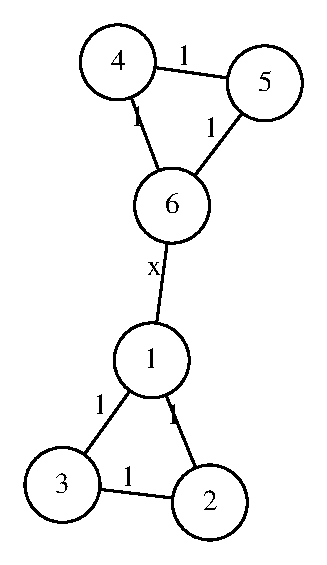
\includegraphics[width=0.8\textwidth]{pic/6point.eps}
	\end{figure}	
		\column{6cm}
  	When $ x < \frac{3}{2}$		
	\begin{equation*}
	 \P = 
		\begin{cases}
			\{\{1,2,3,4,5,6\}\} & \lambda < x \\
			\{\{1,2,3\},\{4,5,6\}\} & x \leq \lambda  < \frac{3}{2} \\
			\{\{1\},\dots,\{6\}\} &  \lambda > \frac{3}{2}
		\end{cases}
	\end{equation*}
    When	$ x = \frac{3}{2}$		
	\begin{equation*}
	 \P = 
	 \begin{cases}
	 	\{\{1,2,3,4,5,6\}\} & \lambda < \frac{3}{2} \\
	 	\{\{1\},\dots,\{6\}\} &  \lambda \geq \frac{3}{2}
	 \end{cases}
	\end{equation*}	
	When	$ x > \frac{3}{2}$
	\begin{equation*}
		\P = 
		\begin{cases}
			\{\{1,2,3,4,5,6\}\} & \lambda <  \frac{3}{2}\\
			\{\{1,6\}, \{2\},\dots\} &  \frac{3}{2} \leq \lambda  < x\\
				\{\{1\},\dots,\{6\}\} &  \lambda \geq x
		\end{cases}
	\end{equation*}				
	\end{columns}
\end{frame}
\section{Algorithms}
\frame{\tableofcontents[currentsection]}
\begin{frame}
\begin{definition}[graph cut function]
$C$ is a subset of $V$:
\begin{align}
f(C) & = \sum_{i\not\in C, j \in C, (i,j) \in E} w_{ij} \\
f[\P] & = \sum_{C \in \P} f(C)
\end{align}
\end{definition}
\begin{theorem}[Principal Sequence of Partition]
\begin{equation}\label{eq:hLambda}
h(\lambda) = \min_{\P \in \Pi(V)} \{ f[\P] - \abs{\P}\lambda \}
\end{equation}
The optimal partitions $\P_1, \dots, \P_k$ for $h(\lambda)$ are nested such that $\P_1 \succeq \P_2 \dots \succeq \P_k$, and we can obtain the hierarchical clustering tree from this sequence.
\end{theorem}
\end{frame}
\begin{frame}
\frametitle{Illustrative Example}
\begin{columns}
\column{5cm}
\begin{figure}
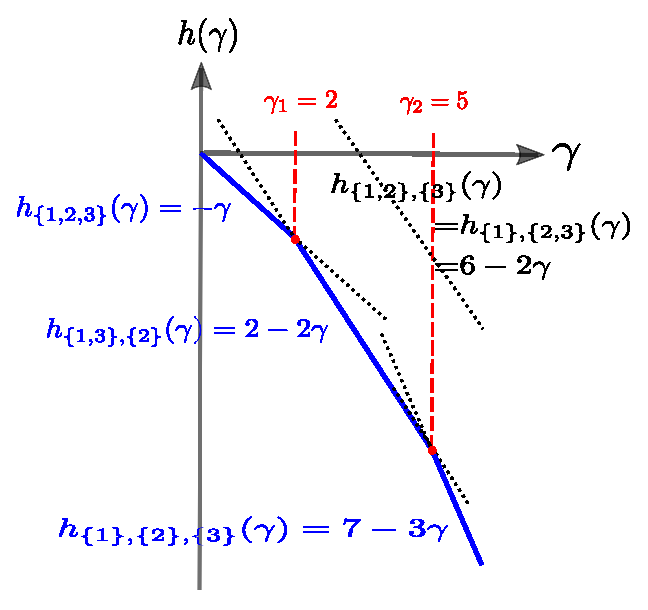
\includegraphics[width=5cm]{pic/dt.eps}
\caption{piecewise linear function $h(\gamma)$}
\end{figure}
\column{5cm}
\begin{align*}
h(\lambda)  & = \min_{\P} h_{\lambda}(\P) \\
h_{\lambda}(\P) & = f[\P] - \abs{\P}\lambda
\end{align*}
\begin{align*}
\P_0  & = \{\{1,2,3\}\} \\
\P_1  & = \{\{1,3\},\{2\}\} \\
\P_2  & = \{\{1\},\{2\},\{3\}\} 
\end{align*}

\end{columns}
\end{frame}
\begin{frame}
\begin{columns}
\column{4cm}
\begin{figure}[!ht]
\centering
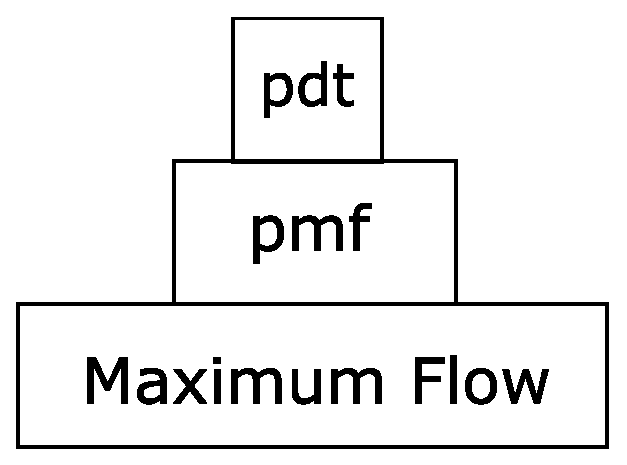
\includegraphics[width=4cm]{pic/pdt.eps}
\caption{pyramid structure of graph-based info-clustering algorithm}\label{fig:ps}
\end{figure}
\column{6cm}
\begin{enumerate}
\item parametric Dilworth truncation: $\min \{f[\P] -\lambda \abs{\P}\}$
\item parametric maximum flow: $\min_{t\in C} \{f(C) - \lambda - y^{\lambda}(C)\}$
\item maximum flow
\end{enumerate}
Achievable time complexity: $\abs{V}^3 \sqrt{\abs{E}}$
% For push-relabel algorithm, \mathrm{MF}(G(V,E)) = \abs{V}^2 E
\end{columns}
\end{frame}
\begin{frame}
	\frametitle{Solving $\min_{t\in C} \{f(C) - \lambda - y^{\lambda}(C)\}$}
	\begin{columns}
    \column{5.3cm}
    \begin{itemize}
	\item $y^{\lambda}$ is a vector
	\item $y^{\lambda}_i = \min\{a_i - \lambda, b_i\}$ 
	\item $y(C) = \sum_{i \in C} y_i$	
	\item $g_{\lambda}(T) = f(T) - \lambda - y^{\lambda}(T)$
	\item $T^{\lambda} = \argmin_{t\in V} g_{\lambda}(T)$
	\end{itemize}
	\begin{theorem}[Principal Sequence]
		\begin{align}\notag
			T^{\lambda} & =\begin{cases}
				T_0 & \lambda < \lambda_1 \\
				T_i & \lambda_i \leq \lambda < \lambda_{i+1}\\
				T_k & \lambda \geq \lambda_{k}
			\end{cases} \\
				T_k & \subsetneq  \dots \subsetneq T_1 \subsetneq T_0 \label{eq:Alambda}				
		\end{align}
    \end{theorem}
	\column{4.7cm}
	\algsetup{linenosize=\tiny}
	\begin{algorithm}[H]
	\caption{
    \ifbeamer
    {\footnotesize
    \fi
    Parametric Computing of $T^{\lambda} = \argmin_{t\in T} g_{\lambda}(T)$
    \ifbeamer
    }
    \fi
    }\label{alg:pmfT}
    \ifbeamer
    {\tiny
    \fi
	\begin{algorithmic}[1]
		\REQUIRE set $V$, $t \in V$, function $g_{\lambda}$ whose domain is $V$.
		\ENSURE An ordered array \textbf{L} which contains $\lambda_1, \dots \lambda_k$ and a reversely ordered array $T^{\lambda}$ which contains $T_0,\dots, T_k$. (defined in equation \eqref{eq:Alambda})
		\STATE \textbf{L}, $A^{\lambda} \leftarrow$ empty arrays of size $\abs{V}$
		\STATE $Q \leftarrow \argmin_{A\in V} g_{-\epsilon}(A), P \leftarrow \{ t \}$ \label{alg:uini}
		\STATE add $Q$ and $P$ to $T^{\lambda}$
		\STATE \texttt{Split}$(Q,P)$
		\FUNCTION{\texttt{Split}$(Q,P)$}
		\STATE Let $\tilde{\lambda}_2$ be the solution to $g_{\lambda}(Q) =  g_{\lambda}(P)$
		\STATE $h' = g_{\tilde{\lambda}_2}(Q)$
		\STATE $P' =\argmin_{A\in V} g_{\tilde{\lambda}_2}(A)$  \label{alg:Pap}
		\IF{$ g_{\tilde{\lambda}_2}(P') = h'$}
		\STATE add  $\tilde{\lambda}_2$ to $\mathbf{L}$
		\ELSE
		\STATE add $P'$ to $T^{\lambda}$ \label{alg:addP}
		\STATE \texttt{Split}$(Q,P')$
		\STATE \texttt{Split}$(P',P)$
		\ENDIF
		\ENDFUNCTION
	\end{algorithmic}
    \ifbeamer
    }
    \fi
\end{algorithm}	
    \end{columns}
\end{frame}
\begin{frame}
	\frametitle{Illustrative Example}
\begin{columns}
	\column{5cm}
	\begin{figure}
		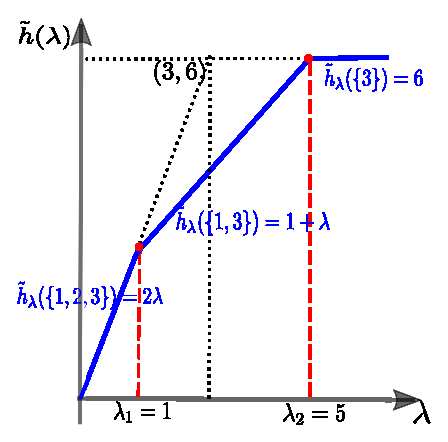
\includegraphics[width=5cm]{pic/example_pst_single.eps}
		\caption{parametric computing illustration}
	\end{figure}
	\column{5cm}
	\begin{align*}
	\tilde{h}(\lambda) &= \min_{t \in T} g_{\lambda}(T)\\
	t & = 3 \\
	y^{\lambda}_i & = -\lambda, i=1,2,3 \\
    \mathbb{L} & = [1, 5, +\infty] \\
	T^{\lambda} &= [\{1,2,3\}, \{1,3\}, \{3\}]
	\end{align*}
\end{columns}	
\end{frame}	
\begin{frame}
	\frametitle{Converting to maximum flow problem}
\begin{columns}
	\column{4cm}
	\begin{figure}
		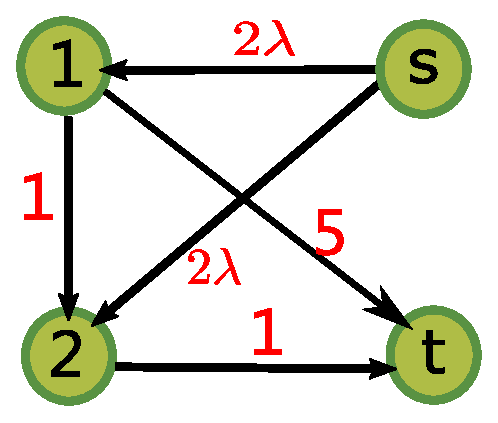
\includegraphics[width=4cm]{pic/example_st.eps}
		\caption{graph $\widetilde{G}$}
	\end{figure}
	\column{6cm}
	\begin{align*}
		& c^{\lambda}(i, j)  = \\ 
		& \begin{cases}
			\max\{0, -y^{\lambda}_i\} &  i = s, j \neq t \\
			w_{it} + \max\{0, y^{\lambda}_i\} & i\neq s, j = t\\
			0 & i = s, j = t\\
			w_{ij} & i \neq s, j \neq t
		\end{cases}
	\end{align*}
\end{columns}	
Minimizing $g_{\lambda}(T)$ is equivalent to solve the maximum flow for $\widetilde{G}$.
\end{frame}	

\section{Experiment}
\frame{\tableofcontents[currentsection]}
\begin{frame}
	\frametitle{How to choose graph weight}
	\framesubtitle{preliminary result}
	\begin{proposition}
		\begin{itemize}
			\item The clustering tree has no stem nodes if and only if
			\begin{equation}
			\frac{f[\P]}{\abs{\P}-1} \geq \frac{\sum_{(i,j) \in E} w_{ij}}{\abs{V}-1}				
			\end{equation}
			holds for any partition $\abs{\P} > 1$.
			\item Let $w_{ij}=0$ if $(i,j)\not\in E$. If $w_{ij} + w_{jk} \geq w_{ki}$ for any different triple $i, j, k \in V$, then the clustering tree has no stem nodes.
			\item Suppose $S_1, S_2 $ are complete graph with size $n$ equal weight $w_{ij}=n$. There are $m$ edges between the two graphs and all inter-connection edges have equal weight 1. Then for $V=S_1\cup S_2$, we have
			\begin{equation}
				I(Z_V) = \begin{cases}
					m & m <\frac{n^2}{2}, S_1,S_2 \textrm{ are non-trivial cluster} \\
					\frac{m+n^2(n-1)}{2n-1} & m\geq \frac{n^2}{2}, \textrm{ only trivial cluster exists} 
				\end{cases}
			\end{equation}
				
		\end{itemize}
	\end{proposition}
\end{frame}
\begin{frame}
\begin{figure}[!ht]
\begin{subfigure}{\textwidth}
\centering
\IfFileExists{experiment/data_clustering/plot_art/build/4part.eps}
{\includegraphics[width=11cm]{experiment/data_clustering/plot_art/build/4part.eps}}
{\includegraphics[width=12cm]{pic/4part.eps}} % not up-to-date

\caption{Illustrative example from four Gaussians}\label{fig:4p}
\end{subfigure}
\begin{subfigure}{\textwidth}
\centering
\IfFileExists{experiment/data_clustering/plot_art/build/3circle.eps}
{\includegraphics[width=11cm]{experiment/data_clustering/plot_art/build/3circle.eps}}
{\includegraphics[width=12cm]{pic/3circle.eps}} % not up-to-date
\caption{Illustrative example from three circles}\label{fig:3c}
\end{subfigure}
\end{figure}
\end{frame}
\begin{frame}
\frametitle{empirical comparison}
\begin{table}[!ht]
\centering
\InputIfFileExists{compare_3.tex}{}{}
\caption{clustering accuracy for info-clustering and existing algorithms}
\end{table}
\end{frame}
\begin{frame}
\frametitle{Info-clustering in hierarchical community detection problem}
\begin{figure}
	\centering
	\begin{subfigure}{0.45\textwidth}
		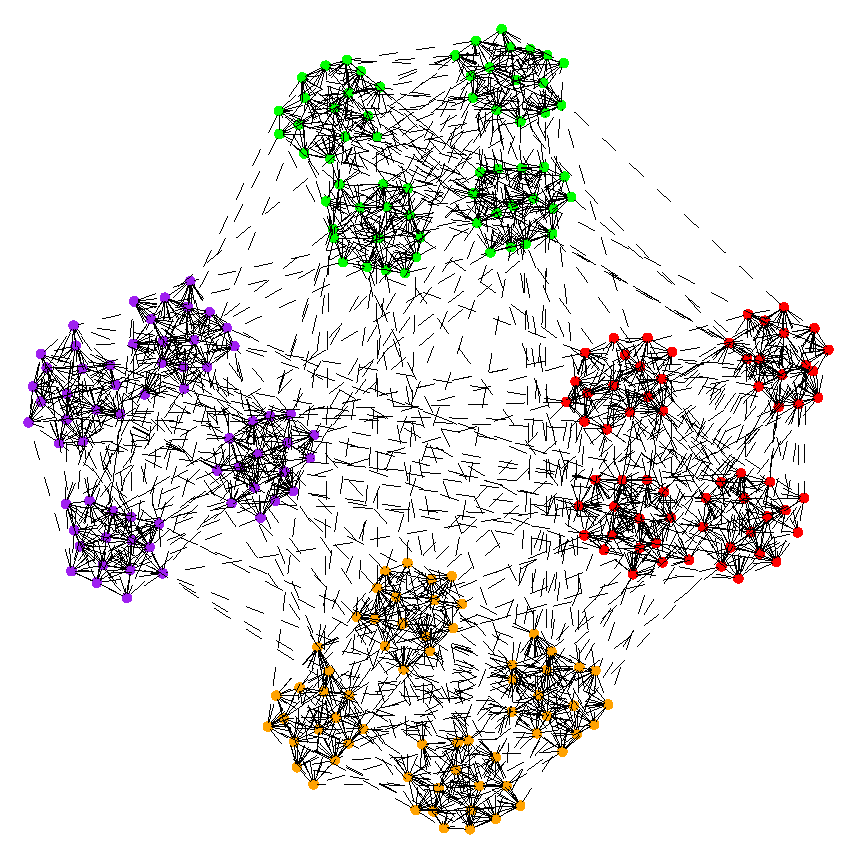
\includegraphics[width=\textwidth]{pic/two_level.eps}
		\caption{a community with two hierarchical levels}\label{fig:c1}
	\end{subfigure}
	\begin{subfigure}{0.45\textwidth}
		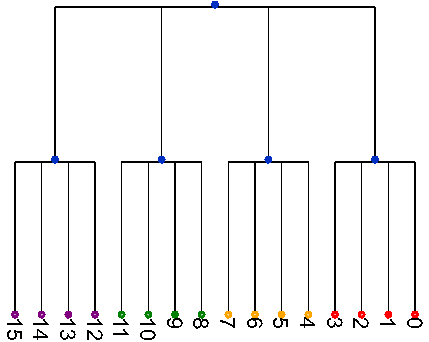
\includegraphics[width=\textwidth]{pic/tree_info-clustering.pdf}
		\caption{hierarchical tree obtained by graph-based info-clustering for left figure. The tree leaves with the same ancestor are merged for clarity.}\label{fig:c2}
	\end{subfigure}
	\caption{Community Detection Experiment Illustration}
\end{figure}
\end{frame}
\begin{frame}
	\begin{block}{model parameter}
	\begin{description}
	  \item[$z_{\mathrm{in}_1}$] average node degree within micro community;
	  \item[$z_{\mathrm{in}_2}$] average node degree between different micro communities but within one macro community;  
	  \item[$z_{\mathrm{out}}$] average node degree between different macro communities
    \end{description}
    Robinson-Foulds distance measure between two trees;    
    {\footnotesize compared with GN(Girvan-Newman) and BHCD(Bayesian hierarchical community detection).
	}
    \end{block}
\begin{figure}
	\centering
	\begin{subfigure}{0.33\textwidth}
		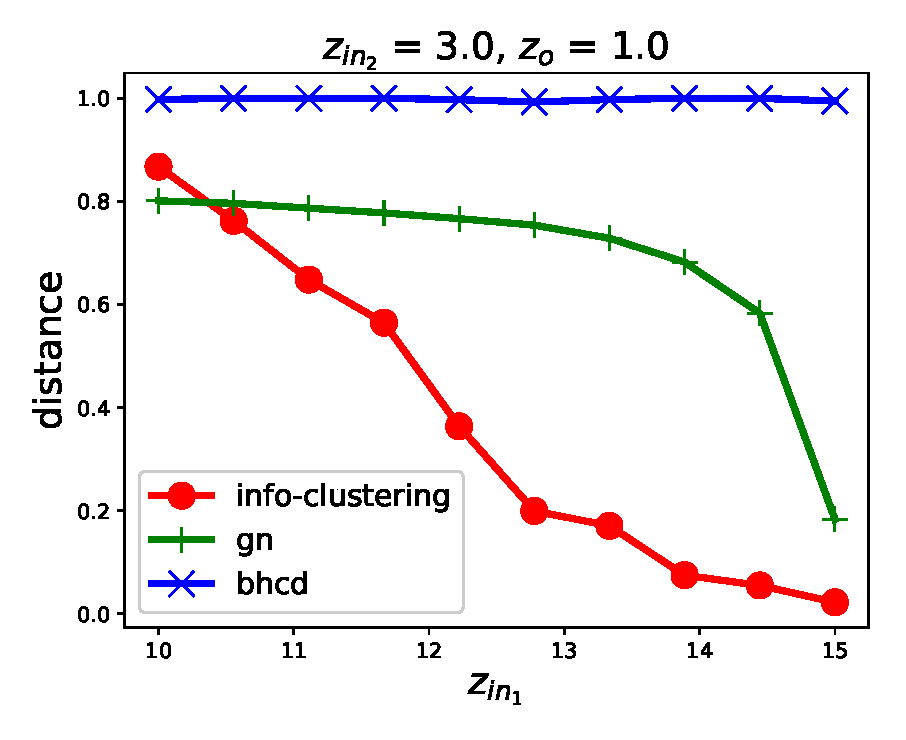
\includegraphics[width=\textwidth]{pic/z_in_1.eps}
		\caption{}
	\end{subfigure}~
	\begin{subfigure}{0.33\textwidth}
		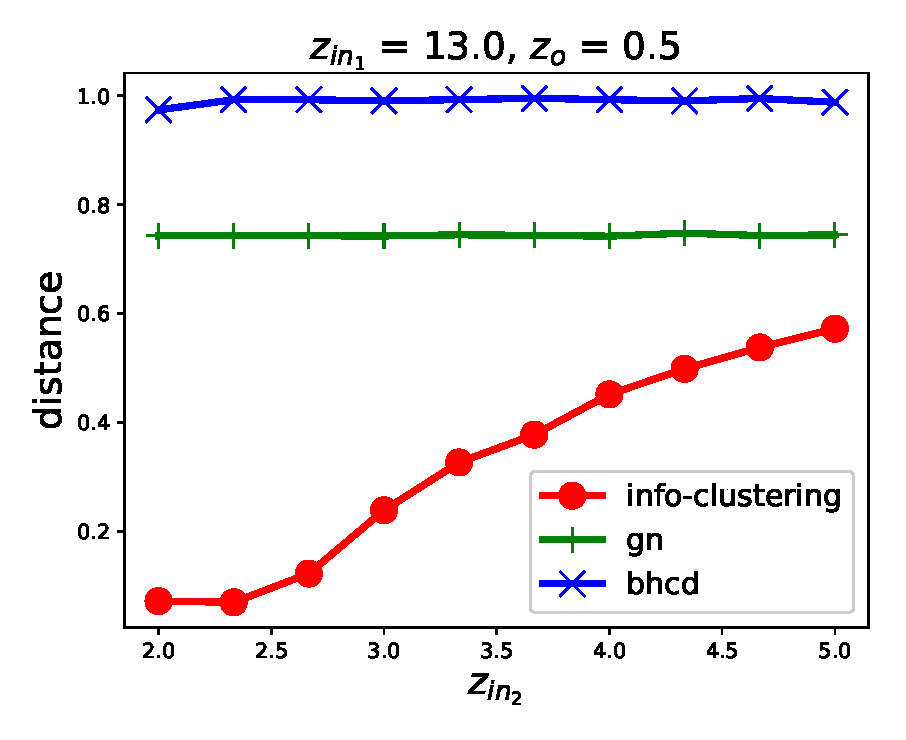
\includegraphics[width=\textwidth]{pic/z_in_2.eps}
		\caption{}
	\end{subfigure}~
	\begin{subfigure}{0.33\textwidth}
		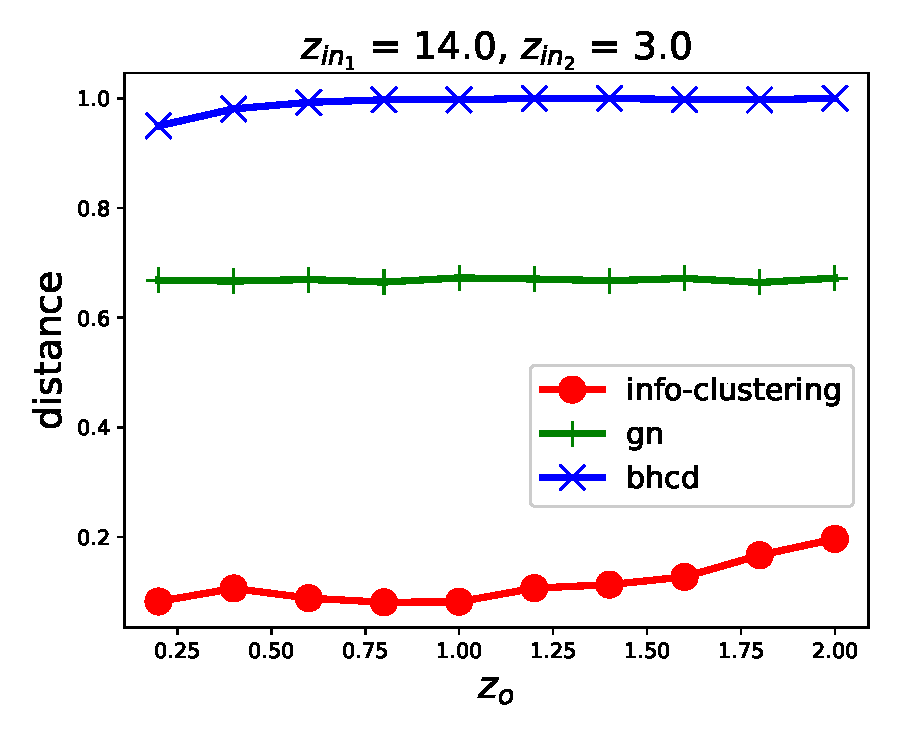
\includegraphics[width=\textwidth]{pic/z_o.eps}
		\caption{}
	\end{subfigure}
	\caption{{\scriptsize Distance comparison between different hierarchical community detection method.}}\label{fig:cdr}	
\end{figure}    
\end{frame}
\section{Conclusion and Contribution}
\begin{frame}
\frametitle{Conclusion}
\begin{itemize}
\item propose graph-based info-clustering method
\item propose a parametric computing scheme to get the hierarchical structure of given graph 
\item apply graph-based info-clustering to cluster dataset and find structure of community
\end{itemize}
\end{frame}
\section{Reference}
\begin{frame}
\frametitle{Reference}
\begin{thebibliography}{9}
\bibitem{ic} Chung Chan, \newblock Info-Clustering: A Mathematical Theory for Data Clustering
\newblock  IEEE Transactions on Molecular, Biological and Multi-Scale Communications, June 2016
\bibitem{pin}  Chung Chan, \newblock Info-Clustering: An Efficient Algorithm by Network Information Flow
\newblock 2017 Information Theory and Applications Workshop (ITA)
\bibitem{mac} Kiyohito Nagano \newblock Minimum Average Cost Clustering \newblock NIPS 2010
\bibitem{RN4}
Vladimir Kolmogorov.
\newblock A faster algorithm for computing the principal sequence of partitions
of a graph.
\newblock {\em Algorithmica}, 56(4):394--412, 2010.
\end{thebibliography}
\end{frame}
\end{document}
